\documentclass{beamer}
\usetheme{Madrid}
\usecolortheme{default}
\useoutertheme{split}
\useinnertheme{circles}
\usepackage{xcolor}
\usepackage{mathrsfs}
\usepackage{amsmath}
\usepackage{amssymb}
\usepackage{booktabs}
\usepackage{hyperref}
\usepackage{animate}
\usepackage{caption}
\usepackage{tikz}
\usetikzlibrary{arrows.meta, positioning, shapes.geometric, shadows}
\captionsetup[figure]{font=tiny}

\usepackage[
    backend=biber,
    style=alphabetic,
    sorting=ynt
]{biblatex}
\addbibresource{bibliography.bib}

% --- Couleurs CS ---
\definecolor{CSred}{RGB}{160,32,60}
\definecolor{CSgrey}{RGB}{136,121,150}
\definecolor{UPSred}{RGB}{97,21,58}
\setbeamercolor{titlelike}{bg=CSred}
\setbeamerfont{title}{series=\bfseries}
\setbeamercolor{palette primary}{bg=CSred,fg=white}
\setbeamercolor{palette secondary}{bg=CSred,fg=white}
\setbeamercolor{palette tertiary}{bg=CSgrey,fg=white}
\setbeamercolor{palette quaternary}{bg=CSgrey,fg=white}
\setbeamercolor{structure}{fg=CSgrey}

\title[Manipulation Detection]{Probabilistic Detection of Market Manipulation}
\subtitle{Research Project - Final Presentation}
\author[Jamal, Martini]{Adonis~Jamal \and Jean Martini\\Supervisor: Damien Challet\\Tutor: Lionel Gabet}
\institute[CentraleSupélec]{CentraleSupélec -- MICS Laboratory}
\date[April 14, 2026]{April 14, 2026}

\titlegraphic{
    
\includegraphics[height=0.8cm]{img/logo_cs}
    \hspace{2cm}
    
\includegraphics[height=0.8cm]{img/logoMICS.png}
}

\begin{document}

% FOR THIS PRESENTATION
% We need:
% Introduce project context, motivation, objectives, and outline of the presentation.
% Then explain the importance of detecting market manipulation and the challenges involved, approaches to market manipulation (spoofing, etc)
% State of the art in market manipulation detection, and the gap our research aims to fill.
% Compared to the other presentations, which were more focused on the technical details of the models and the methodology
% This presentation should be more focused on the results and their implications, as well as the broader context of market manipulation detection.
% We should also discuss the limitations of our approach and potential future work, as well as the practical implications of our findings for market participants and regulators.
% Since we have 30 minutes, and a lot of information to cover, we should use the tikz diagram to explain the overall architecture of our approach, and follow it throughout the presentation to explain how the different components fit together.
% Once that's done, we should present the results of our experiments, 




\frame{\titlepage}

\begin{frame}
    \frametitle{Table of Contents}
    \tableofcontents
\end{frame}

% ==============================================================================
% SECTION 1: INTRODUCTION
% ==============================================================================
\section{Introduction}


\begin{frame}{}
    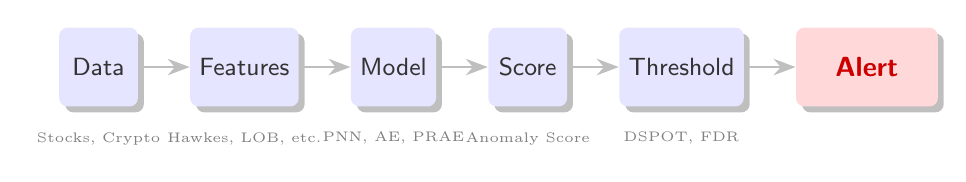
\begin{tikzpicture}[
        % Définition des styles pour une réutilisation facile
        node distance = 0.65cm, % Distance entre les blocs
        every node/.style = {font=\sffamily\small}, % Police sans-serif
        % Style des blocs standards
        block/.style = {
            rectangle, 
            draw=none, 
            fill=blue!10, 
            text=black!80, 
            minimum width=1cm, 
            minimum height=1cm, 
            rounded corners=3pt,
            drop shadow,
            align=center
        },
        % Style spécifique pour l'alerte (mise en évidence)
        alert/.style = {
            rectangle, 
            draw=none, 
            fill=red!15, 
            text=red!80!black, 
            minimum width=1.8cm, 
            minimum height=1cm, 
            rounded corners=3pt,
            drop shadow,
            align=center,
            font=\sffamily\bfseries
        },
        % Style des flèches
        arrow/.style = {
            -{Stealth[scale=1.2]}, % Pointe de flèche moderne
            thick, 
            draw=gray!50
        }
    ]

        % 1. Placement des nœuds (Nodes)
        \node (data)   [block] {Data};
        \node (feat)   [block, right=of data] {Features};
        \node (model)  [block, right=of feat] {Model};
        \node (score)  [block, right=of model] {Score};
        \node (thresh) [block, right=of score] {Threshold};
        \node (alert)  [alert, right=of thresh] {Alert};

        % 2. Tracé des flèches (Arrows)
        \draw [arrow] (data) -- (feat);
        \draw [arrow] (feat) -- (model);
        \draw [arrow] (model) -- (score);
        \draw [arrow] (score) -- (thresh);
        \draw [arrow] (thresh) -- (alert);

        % 3. (Optionnel) Ajout de légendes ou annotations
        % Exemple : Annotation sous le seuil
        \node [below=0.2cm of data, font=\tiny, text=gray] {Stocks, Crypto};
        \node [below=0.2cm of feat, font=\tiny, text=gray] {Hawkes, LOB, etc.};
        \node [below=0.2cm of model, font=\tiny, text=gray] {PNN, AE, PRAE};
        \node [below=0.2cm of score, font=\tiny, text=gray] {Anomaly Score};
        \node [below=0.2cm of thresh, font=\tiny, text=gray] {DSPOT, FDR};

    \end{tikzpicture}
\end{frame}


% ==============================================================================
% SECTION 4: CONCLUSION
% ==============================================================================
\section{}
\begin{frame}{}
    \centering
    \LARGE{Thank you for your attention!}
\end{frame}


% ==============================================================================
% SECTION: BIBLIOGRAPHY
% ==============================================================================
\begin{frame}[allowframebreaks]
    \frametitle{Bibliography}
    \nocite{*}
    \printbibliography
\end{frame}


% ==============================================================================
% SECTION: APPENDIX
% ==============================================================================
\appendix
\section{Appendix}
\begin{frame}{}
\end{frame}

\end{document}